\subsection{วางโครงสร้างของระบบพื้นฐาน}
โครงสร้างระบบพื้นฐานของหุ่นยนต์ฮิวมานอยด์ UTHAI เป็นการวางระบบให้ผู้วิจัยสามารถที่จะช่วยกันพัฒนาได้
และเพื่อทำให้มีความเป็นระบบระเบียบ ง่ายต่อการแก้ไข ปรับปรุง
ซึ่งผู้วิจัยได้ออกแบบส่วนการทำงานต่างๆออกเป็นสามส่วน ตามหน้าที่การทำงาน คือ

\subsubsection*{Hardware Devices}
เป็นส่วนของอุปกรณ์ฮาร์ดแวร์ที่ใช้งานกับหุ่นยนต์ฮิวมานอยด์ ยกตัวอย่างเช่น ตัวขับเคลื่อน กล้อง ไมโครโฟน ลำโพง
หรืออื่นๆ ซึ่งในส่วนนี้สามารถเปลี่ยนฮาร์ดแวร์จริงๆเป็นระบบจำลองได้

\subsubsection*{Hardware Services}
เป็นส่วนของซอฟต์แวร์ที่ช่วยทำให้อุปกรณ์ฮาร์ดแวร์สามารถติดต่อสื่อสารกับระบบพื้นฐานของหุ่นยนต์ฮิวมานอยด์ UTHAIได้
ซึ่งจะช่วยทำให้การส่งข้อมูลเป็นมาตรฐานเดียวกัน

\subsubsection*{Communication}
เป็นส่วนของการติดต่อสื่อสารระหว่างซอฟต์แวร์กับฮาร์ดแวร์ผ่านระบบพื้นฐานของหุ่นยนต์ฮิวมานอยด์ ซึ่งจะคอยจัดการให้ข้อมูลทุกอย่างสามารถเชื่อมต่อกันได้
\begin{figure}[!ht]
	\centering
	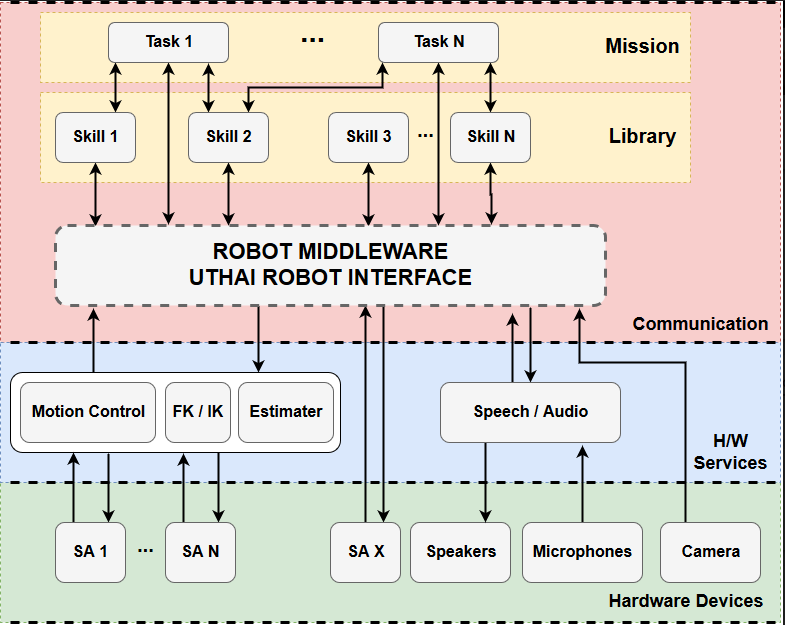
\includegraphics[width=0.8\textwidth]{chapter3/images/uthai_diagram.png}
	\caption{โครงสร้างพื้นฐานของหุ่นยนต์ฮิวมานอยด์ UTHAI}
	\label{fig:uthai_diagram}
\end{figure}

\clearpage
\begin{figure}[!ht]
	\centering
	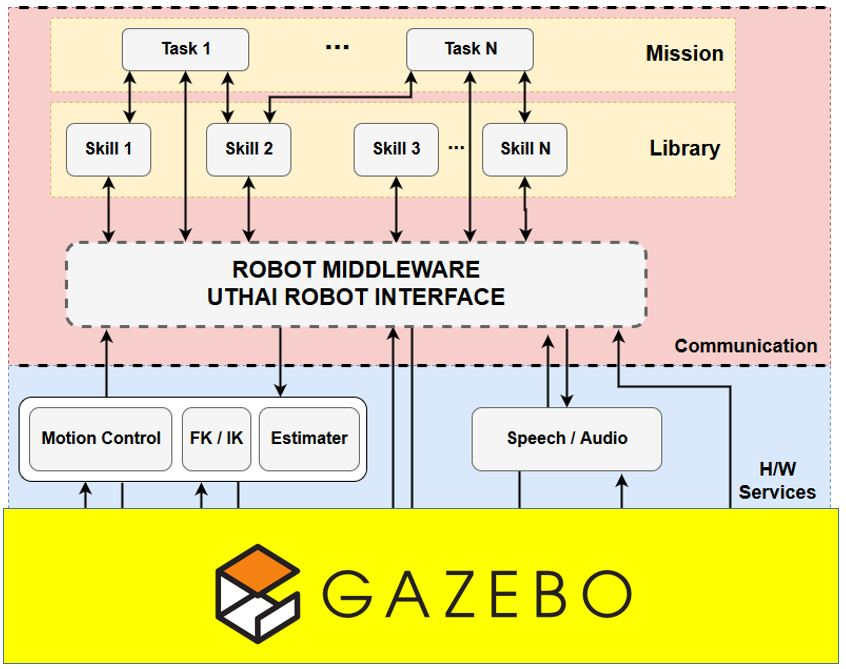
\includegraphics[width=0.85\textwidth]{chapter3/images/platform3.JPG}
	\caption{ภาพการเปลี่ยนส่วนของฮาร์ดแวร์เป็นระบบจำลอง}
\end{figure}
\begin{figure}[!ht]
	\centering
	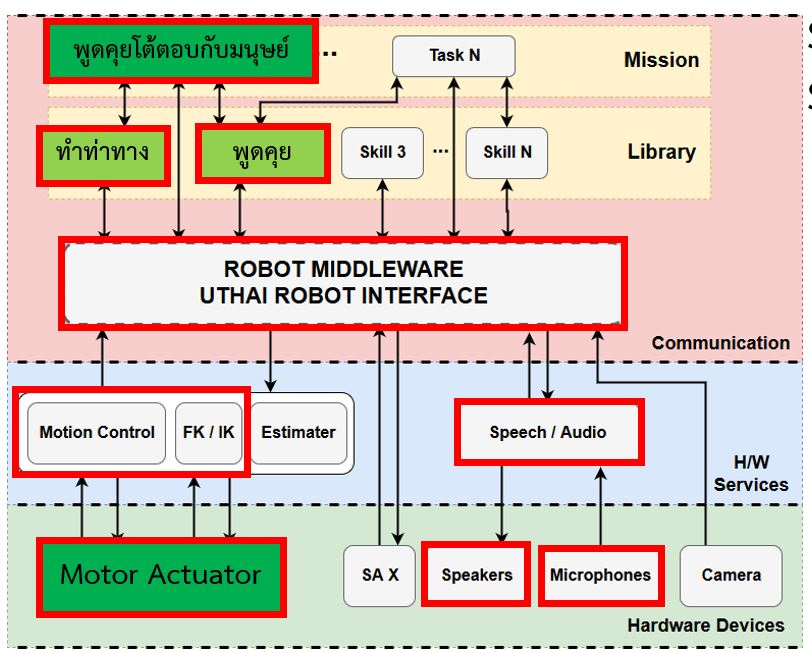
\includegraphics[width=0.85\textwidth]{chapter3/images/platform2.JPG}
	\caption{ตัวอย่างการนำโครงสร้างพื้นฐานไปประยุกต์ใช้ ในแอพลิเคชันการพูดคุยโต้ตอบกับมนุษย์}
\end{figure}

\clearpage
\subsection{ออกแบบสถาปัตยกรรมของหุ่นยนต์}
หลักการออกแบบสถาปัตยกรรมของหุ่นยนต์ฮิวมานอยด์ UTHAI จะออกแบบระบบให้อยู่บนระบบพื้นฐาน ROS
เนื่องจากการใช้กรอบการทำงานที่มีประสิทธิภาพ และความยืดหยุ่นสูง จะช่วยทำให้สามารถปรับเปลี่ยนระบบการควบคุมของหุ่นยนต์ฮิวมานอยด์ได้ง่ายและรวดเร็ว
การออกแบบหน่วยประมวลผลนั้นมีหลากหลายรูปแบบ ดังที่กล่าวไปในบทที่ 2 สำหรับในงานวิจัยครั้งนี้ผู้วิจัยได้ศึกษาและพบกว่าสถาปัตยกรรมที่เหมาะสมกับหุ่นยนต์ฮิวมานอยด์ UTHAI
จะมีลักษณะใกล้เคียงกับหุ่นยนต์ฮิวมานอยด์ Robotis OP3 ดังรูปที่ \ref{fig:op3_argitec} ดังนั้นแล้วผู้วิจัยจึงได้แบ่งการประมวลผลออกเป็น 2 ส่วนคือ
\begin{enumerate}[label=\arabic*, leftmargin=1.5cm]\setlength\itemsep{-0.25em}
	\item หน่วยประมวลผลควบคุมระดับสูง (High Level Controller)
	\item หน่วยประมวลผลควบคุมระดับต่ำ (Low Level Controller)
\end{enumerate}
\begin{figure}[!ht]
	\centering
	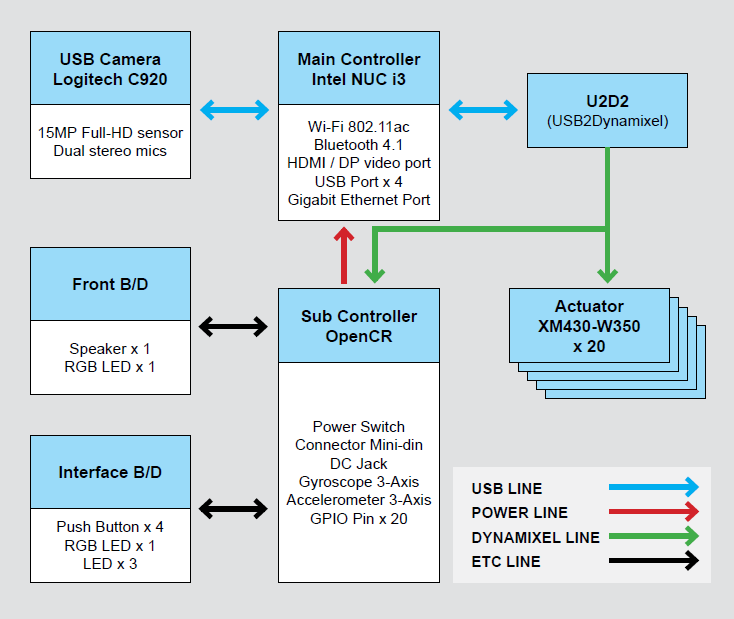
\includegraphics[width=0.6\textwidth]{chapter3/images/op3_029.png}
	\caption{สถาปัตยกรรมของหุ่นยนต์ Robotis OP3}
	\label{fig:op3_argitec}
\end{figure}
\begin{figure}[!ht]
	\centering
	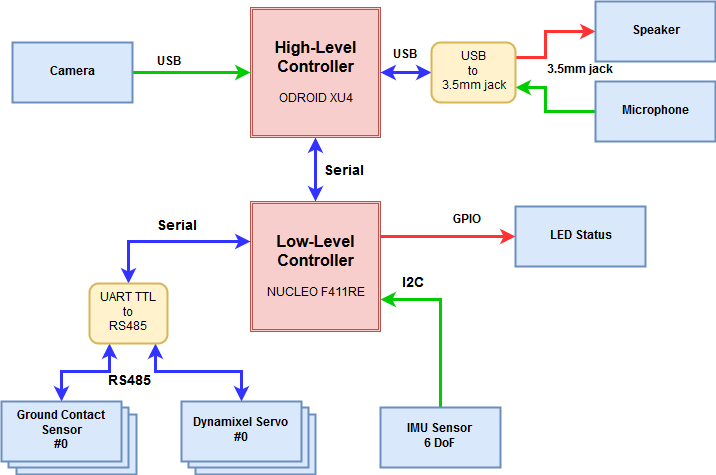
\includegraphics[width=0.7\textwidth]{chapter3/images/uthai_argitec.png}
	\caption{สถาปัตยกรรมของหุ่นยนต์ฮิวมานอยด์ UTHAI}
	\label{fig:uthai_argitec}
\end{figure}

\clearpage
\subsubsection{หน่วยประมวลผลควบคุมระดับสูง (High level controller)}
ระบบควบคุมหลักของหุ่นยนต์ฮิวมานอยด์ UTHAIนั้นจะอยู่ที่หน่วยประมวลผลขั้นสูง ใช้เป็นบอร์ดคอมพิวเตอร์ ODROID-XU4 ตัวประมวลผลหลักนี้
ทำหน้าที่ในการคำนวณเส้นทางการเดิน ทำให้หุ่นยนต์มีเสถียรภาพในการเดิน ตรวจการขัดกันของโครงสร้างของหุ่นยนต์
รวมไปถึงรับค่าข้อมูลตำแหน่ง ความเร็วจากข้อต่อ หลังจากนั้นจะทำการนำค่าทั้งหมดที่ได้จากการคำนวณ
มาแปลงให้อยู่ในรูปของชุดข้อมูล แล้วส่งออกไปให้ระบบกลาง (ROS) ในการส่งต่อไปให้อุปกรณ์อื่นต่อไป

\begin{figure}[ht]
	\centering
	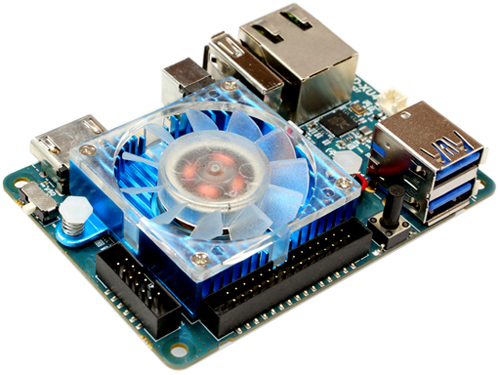
\includegraphics[width=0.45\textwidth]{chapter3/images/odroid_xu4.jpeg}
	\caption{บอร์ดคอนโทรลเลอร์ Odroid XU4}
	\label{fig:controller_xu4}
\end{figure}

\subsubsection{หน่วยประมวลผลควบคุมระดับต่ำ (Low level controller)}
ระบบควบคุมขั้นต่ำเป็นหน่วยประมวลผลที่รองลงมาจาก บอร์ดคอมพิวเตอร์ โดยใช้บอร์ดไมโครคอลโทรเลอร์ Nucleo F411RE
เป็นหน่วยประมวลผลขั้นต่ำ สำหรับในการติดต่อกับอุปกรณ์อิเล็กทรอนิกส์ต่างๆ ที่อยู่ภายในตัวของหุ่นยนต์ เช่น
ค่าเซนเซอร์ที่ฝ่าเท้าซึ่งสามารถบอกได้ว่าควรใช้สมการไหนในการคำนวณพลวัต หรือค่าของเซนเซอร์หน่วยวัดความเฉื่อยมีความสำคัญมาก
ในการทำให้หุ่นยนต์ฮิวมานอยด์เดินได้อย่างมีเสถียรภาพ เมื่ออ่านค่าเซนเซอร์ต่างๆได้แล้ว
หน่วยประมวลผลขั้นต่ำจะนำค่าที่ได้จากการอ่านเซนเซอร์เหล่านี้แปลงให้อยู่ในลักษณะของชุดข้อมูล แล้วส่งออกไปในระบบกลาง (ROS)
นอกเหนือจากนี้หน่วยประมวลผลขั้นต่ำยังทำหน้าที่รับค่าคำสั่งมาจากระบบกลาง ในการสั่งงานให้หุ่นยนต์มีท่าทางต่างๆได้

\begin{figure}[ht]
	\centering
	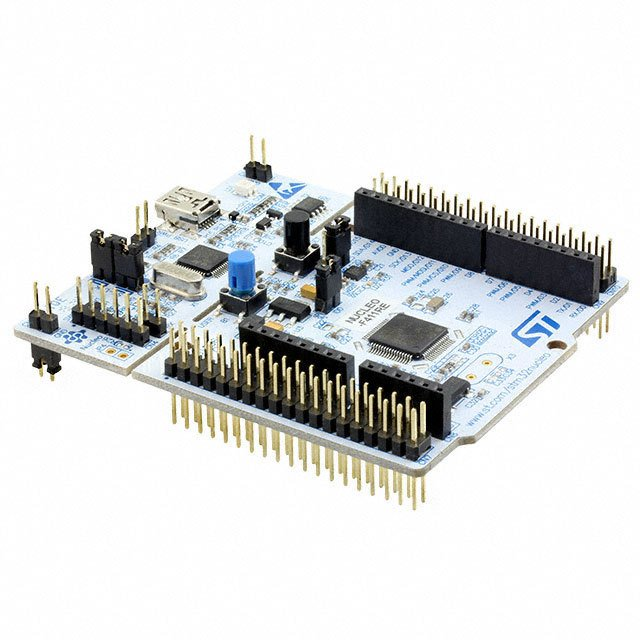
\includegraphics[width=0.45\textwidth]{chapter3/images/nucleo_f411re.jpeg}
	\caption{บอร์ดคอนโทรลเลอร์ Nucleo F411RE}
	\label{fig:controller_f411re}
\end{figure}


%%%%%%%%%%%%%%%%%%%%%%%%%%%%%%%%%%%%%%%%%%%%%%%%%%%%%%%%%%%%%%%%%%%%%%%%%%%%%%%

\clearpage
\subsection{จัดทำคู่มือและเอกสารการใช้งาน}
คู่มือจะเป็นส่วนที่ผู้มาพัฒนาต่อยอดสามารถที่จะอ่านทำความเข้าใจได้ โดยจะเขียนให้อยู่ในรูปของไฟล์ 
Markdown (.md) และเก็บเอาไว้ในเว็บไซท์ GitHub ซึ่งเป็นแหล่งรวม Source code ออนไลน์
สามารถเข้าไปดาวน์โหลดไฟล์ลงเครื่องผู้ใช้ แล้วทำการติดตั้งใช้งานได้เลย อีกทั้งผู้ใช้ยังสามารถส่ง Code
ของตัวเองเข้าระบบเพื่อช่วยพัฒนาและเพิ่มประสิทธิภาพในการทำงานของซอฟต์แวร์ของหุ่นยนต์ได้

ส่วนที่ทำคู่มือและเอกสารเบื้องต้นคือ\vspace{-5mm}
\begin{enumerate}[label=\arabic*, leftmargin=1.5cm]\setlength\itemsep{-0.25em}
	\item รายการวัสดุที่ใช้ในการทำหุ่นยนต์ฮิวมานอยด์ UTHAI
	\item รายละเอียดการเชื่อมต่อระหว่างอุปกรณ์ที่อยู่ในตัวหุ่นยนต์
	\item รายละเอียดการประกอบชิ้นส่วนทางกล
	\item รายละเอียดการใช้งานโปรแกรมพื้นฐาน
\end{enumerate}

\subsubsection{รายการวัสดุที่ใช้ในการทำหุ่นยนต์ฮิวมานอยด์ UTHAI}
\begin{table}[ht]
	\centering
	\begin{tabular}{| l | c | c | c|}
		\hline
		รายการ & จำนวน (หน่วย) & บาท/หน่วย & ราคารวม(บาท) \\
		\hline
		===== Processing Unit & - & - & -\\
		Odroid XU4 Embeded Computer & 1 & 3800 & 3800\\
		Shifter Shield for Odoird XU4 & 1 & 1000 & 1000\\
		===== Sensor & - & - & -\\
		Force sensitive Resistor & 8 & 300 & 2400\\
		Electronic Component & 1 & 2000 & 2000\\
		MPU9255 9 Axis IMU Module & 1 & 500 & 500\\
		===== Structure & - & - & -\\
		อุปกรณ์ส่งกำลัง & 1 & 3000 & 3000\\
		ค่าวัสดุ เช่น Filament 3D printer , Carbon Fiber & 1 & 8000 & 8000\\
		สปริง & 14 & 50 & 700\\
		อุปกรณ์สิ้นเปลือง เช่น กระดาษทราย ฯลฯ & 1 & 1000 & 1000\\
		===== อุปกรณ์เสริม Motor Dynamixel & - & - & -\\
		Frame สำหรับต่อพ่วงมอเตอร์ & 4 & 2000 & 8000\\
		Horn Bearing & 4 & 1400 & 5600\\
		อุปกรณ์จ่ายพลังงาน & - & - & -\\
		Power Supply & 1 & 2000 & 2000\\
		Battery Li-Po 4 cell & 1 & 3000 & 3000\\
		===== รวม & - & - & 48000\\
		\hline
	\end{tabular}
	\caption{ตารางแสดงรายการของวัสดุต่าง ๆ}
	\label{tab:matrial_buyer}
\end{table}
ใช้สำหรับแจกแจงค่าใช้จ่ายเบื้องต้นเท่านั้น ไม่สามารถใช้อ้างอิงงบประมาณแบบละเอียดได้

%%%%%%%%%%%%%%%%%%%%%%%%%%%%%%%%%%%%%%%%%%%%%%%%%%%%%%%%%%%%%%%%%%%%%%%%%%%%%%%
% \subsubsection{รายละเอียดการเชื่อมต่อระหว่างอุปกรณ์ที่อยู่ในตัวหุ่นยนต์}
% \subsubsection{รายละเอียดการประกอบชิ้นส่วนทางกล}
% \subsubsection{รายละเอียดการใช้งานโปรแกรมพื้นฐาน}